\documentclass{article}
\usepackage[utf8]{inputenc}
\usepackage{amsmath}
\usepackage{amssymb}
\usepackage{graphicx}
\usepackage{subfig}
\usepackage{tcolorbox}
\usepackage{listings}
\usepackage[left=20mm, right=20mm]{geometry}
\usepackage{enumitem}
\usepackage{amsthm}
\usepackage[hyphens]{url}

\newcommand{\Z}{\mathbb{Z}}
\newcommand{\R}{\mathbb{R}}
\renewcommand{\a}{\land}
\renewcommand{\o}{\lor}
\newcommand{\n}{\neg}
\renewcommand{\i}{\implies}
\newcommand{\p}[1]{\begin{pmatrix} #1\end{pmatrix}}
\newtheorem{theorem}{Theorem}
\newtheorem{lemma}[theorem]{Lemma}

\renewcommand\arraystretch{2}

\title{MATH1064 Assignment 2}
\author{SID: 530328265 - Tutorial: 16.00 TUE}
\date{Due Date: Thursday 2023/10/19}

\begin{document}
	\maketitle
	\section*{1. }
	\begin{enumerate}[label=({\alph*})]
		\item We have the following options.
		\[ (p, q) \in \{(3, 5), (3, 7), (3, 11), (3, 13), (5, 7), (5, 13)\}\]
		From this options, I choose \((p, q) = (5, 13)\).
		We have:
		\[n = pq\]
		Thus, my \(n\) is equal to:
		\[n = pq = 5 \times 13 = 65\]
		\item 
		\begin{figure}[ht]
			\centering
				 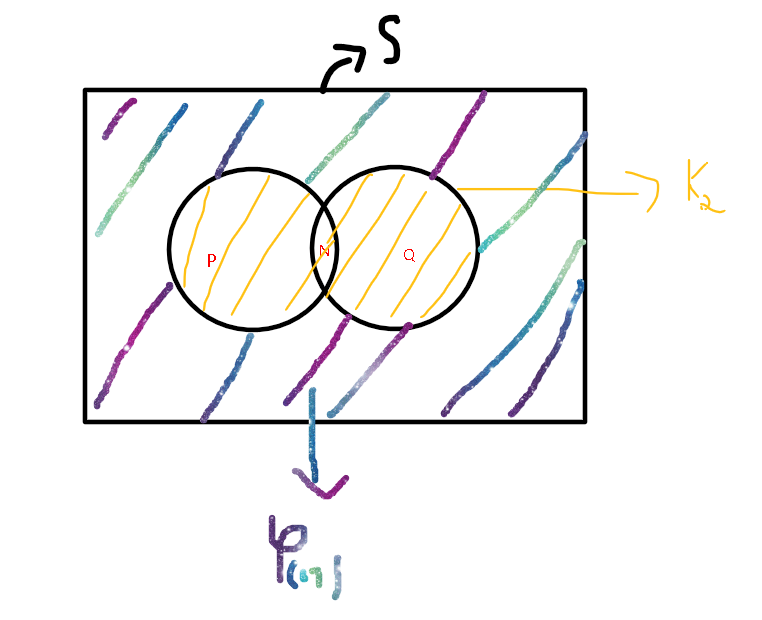
\includegraphics[width=0.4\textwidth]{1b.png} 
				 \caption{Ex: 1b}
				 \label{Ex:1b}
		\end{figure}
		(i). We call \(S = \{k \in \mathbb{N}, 0 < k < n\}\)
	
		We also have: \(n = pq\)

		Then, \(\left| S \right|\) is equal to:
		\begin{equation}
			\left| S \right| = pq - 1 \quad \label{1:b:0}
		\end{equation}

		We call \(P = \{k, p \in \mathbb{N}, 0 < k \leq n, \text{ k is divisible by p} \}\) 

		Then, \(\left| P \right|\) is equal to:
		\begin{equation}
			\left| P \right| = \lfloor (\frac{pq}{p})  \rfloor = q\quad \label{1:b:1}
		\end{equation}
		We call \(Q = \{k, q \in \mathbb{N}, 0 < k \leq n, \text{ k is divisible by q} \}\)

		Then, \(\left| Q \right|\) is equal to:
		\begin{equation}
			\left| Q \right| = \lfloor (\frac{pq}{q})  \rfloor = p\quad \label{1:b:2}
		\end{equation}
		We call \(N = \{k, pq \in \mathbb{N}, 0 < k \leq n, \text{ k is divisible by pq} \}\)

		Then, \(\left| N \right|\) is equal to:
		\begin{equation}
			\left| N \right| = \lfloor (\frac{pq}{pq})  \rfloor = 1\quad \label{1:b:3}
		\end{equation}

		We call \(K_{1} = \{k, p, q \in N, 0 < k \leq n, \text{ k is divisible by p or q}\}\)

		From \eqref{1:b:1}, \eqref{1:b:2} and \eqref{1:b:3}, by the principle of inclusion-exclusion, we can determine the quanitity of numbers that divisible by p or q.
		\begin{equation}
		\left| K_{1} \right| = \left| P \right| + \left| Q \right| - \left| N \right| = p + q - 1 \quad \label{1:b:4}
		\end{equation}

		However, In order to find the number of numbers greater than \(0\)
		but less than pq that are divisible by either \(\text{p or q}\), we subtract the number pq from the set of numbers divisible by \(\text{p or q}\).

		We call \(K_{2} = \{k, p, q \in N, 0 < k < n, \text{ k is divisible by p or q}\}\).

		Then, from \eqref{1:b:4}, we have:
		\begin{equation}
			\left| K_{2} \right| = \left| K_{1} \right| - 1 = p + q - 1 - 1 = p + q - 2 \quad \label{1:b:5}
		\end{equation}

		As the set of all numbers which share a factor with \(pq\) are complement of the set of pq's coprimes, we can determine the number of positive integers \(0 < k < n\) such that \(\gcd{(k, n)} = 1\).

		Thus, from \eqref{1:b:0} and \eqref{1:b:5}, we have:
		\[\varphi(n) = \left| S \right| -  \left| K_{2} \right| = pq - 1 - (p + q - 2) = pq - p - q + 1 = (p - 1)(q - 1) \quad \blacksquare\]
		(ii). From my choice in (a), \(n = 65 \text{ and } (p, q) = (5, 13)\). Thus, my \(\varphi(n)\) is equal to:
		\[\varphi(n) = (p - 1)(q - 1) = (5 - 1)(13 - 1) = 4 \times 12 = 48\]
		\item Choose \(e = 7\) since:
		\[\gcd{(e, \varphi(n))} = \gcd{(7, 48)} = 1\]
		Therefore \(7 \text{ and } 48 \text{ are relatively prime}\).

		Thus, my public key is \((e, n) = (7, 65)\)
		\pagebreak
	\end{enumerate}
	\section*{2. }
	\begin{enumerate}[label=({\alph*})]
		\item Because \(e\) and \(d\) are allowed to be the same number, \(d\) is choosen to be \(7\)
		We have:
		\[ed \equiv 1 \pmod{\varphi(n)} \]
		Then,
		\[7d \equiv 1 \pmod{48}\]
		Then,
		\[7 \times 7 \equiv 1 \pmod{48}\]
		Equal to:
		\[49 \equiv 1 \pmod{48}\]
		Thus, my private key is \((7, 65)\)
	\end{enumerate}
	\section*{3. }
	\begin{enumerate}[label=({\alph*})]
		\item My student number is \(530328265\).Thus my last eight individual digits of my student number is \(30328265\).
		
		To encode the last eight individual digits of my student number, We then calculate the coded message c by finding.
		\[c \equiv m^e \pmod{n} \text{, } 0 \leq c < n \]
		Thus, we have:
		\[c_{1} \equiv m_{1}^e \pmod{n}\]
		Then:
		\[c_{1} \equiv 3^7 \pmod{65} \implies c_{1} = 42\]
		Similar to count \(c_{1}\), we can calculate \(c_{2}\), \(c_{3}\), \(c_{4}\), \(c_{5}\), \(c_{6}\), \(c_{7}\), \(c_{8}\)
		\[c_{2} \equiv 0^7 \pmod{65} \implies c_{2} = 0\]
		\[c_{3} \equiv 3^7 \pmod{65} \implies c_{3} = 42\]
		\[c_{4} \equiv 2^7 \pmod{65} \implies c_{4} = 63\]
		\[c_{5} \equiv 8^7 \pmod{65} \implies c_{5} = 57\]
		\[c_{6} \equiv 2^7 \pmod{65} \implies c_{6} = 63\]
		\[c_{7} \equiv 6^7 \pmod{65} \implies c_{7} = 46\]
		\[c_{8} \equiv 5^7 \pmod{65} \implies c_{8} = 60\]
		\item To decode a message c using my private key \((7, 65)\), we calculate m using the following equation.
		\[m \equiv c^d \pmod{n} \text{, } 0 \leq m < n\]
		Thus, we have:
		\begin{equation}
			m_{1} \equiv c_{1}^d \pmod{n} \quad \label{4:a:0}
		\end{equation}
		Then:
		\[m_{1} \equiv 42^7 \pmod{65}\]
		We have: 
		\[42 ^ 7 \equiv (42 ^ 2 \times 42 ^ 2 \times 42 ^ 2 \times 42) \pmod{65}\]
		Which equal to:
		\begin{equation}
			42 ^ 7 \equiv (9 \times 9 \times 9 \times 42) \pmod{65} \quad \label{3:b:1}
		\end{equation}
		From \eqref{3:b:1}, we have:
		\[42 ^ 7 \equiv 3 \pmod{65}\]
		Thus, \(m_{1} = 3\)

		Similar to count \(m_{1}\), we can calculate \(m_{2}\), \(m_{3}\), \(m_{4}\), \(m_{5}\), \(m_{6}\), \(m_{7}\), \(m_{8}\)
		\[m_{2} \equiv 0^7 \pmod{65} \implies m_{2} = 0\]
		\[m_{3} \equiv 42^7 \pmod{65} \implies m_{3} = 3\]
		\[m_{4} \equiv 63^7 \pmod{65} \implies m_{4} = 2\]
		\[m_{5} \equiv 57^7 \pmod{65} \implies m_{5} = 8\]
		\[m_{6} \equiv 63^7 \pmod{65} \implies m_{6} = 2\]
		\[m_{7} \equiv 46^7 \pmod{65} \implies m_{7} = 6\]
		\[m_{8} \equiv 60^7 \pmod{65} \implies m_{8} = 5\]
	\end{enumerate}
	\section*{4. }
	\begin{enumerate}[label=({\alph*})]
		\item I find a friend that have different public key from mine. His public key is \((e, n) = (5, 39)\)
		\item Because my friend's public key is \((5, 39)\) so \(e = d = 5\) and \(n = 39\)
		
		I choose \textbf{EUCLID} is the last name of a famous mathematician from history.

		Then, convert each letter of \textbf{EUCLID} to a 2-digit number (i.e A = 1, B = 2, ..., Z = 26). Thus, we have the table below.
		\begin{center}
			\begin{tabular}{| c | c ||| c | c |||c | c ||| c | c |}
				\hline 
				Letter &  Number & Letter & Number & Letter & Number & Letter & Number\\
				\hline
				A & 1 & H & 8 & O & 15 & V & 22\\
				B & 2 & I & 9 & P & 16 & W & 23\\
				C & 3 & J & 10 & Q & 17 & X & 24\\
				D & 4 & K & 11 & R & 18 & Y & 25\\
				E & 5 & L & 12 & S & 19 & Z & 26\\
				F & 6 & M & 13 & T & 20 &   &    \\
				G & 7 & N & 14 & U & 21 &   &    \\
				\hline
			\end{tabular}
		\end{center}
		From the table, we can see that \(E = 5\), \(U = 21\), \(C = 3\), \(L = 12\), \(I = 9\), \(D = 4\).

		Thus, when convert \textbf{EUCLID} to 2-digit number, we have,
		\[\textbf{EUCLID} \implies 5|21|3|12|9|4\]

		Then, I will encode this name by using friend's public key \((5, 39)\) by using:
		\[c \equiv m^e \pmod{n} \text{, } 0 \leq c < n\]
		Which equal to:
		\[c \equiv m^5 \pmod{39} \text{, } 0 \leq c < 39\]
		1. Encode E:
		\[E = 5 \implies c_{E} \equiv 5 ^ 5 \pmod{39} \implies c_{E} = 5\]
		2. Encode U:
		\[U = 21 \implies c_{U} \equiv 21 ^ 5 \pmod{39} \implies c_{U} = 21\]
		3. Encode C:
		\[C = 3 \implies c_{C} \equiv 3 ^ 5 \pmod{39} \implies c_{C} = 9\]
		4. Encode L:
		\[L = 12 \implies c_{L} \equiv 12 ^ 5 \pmod{39} \implies c_{L} = 12\]
		5. Encode I:
		\[I = 9 \implies c_{I} \equiv 9 ^ 5 \pmod{39} \implies c_{I} = 3\]
		6. Encode D:
		\[D = 4 \implies c_{D} \equiv 4 ^ 5 \pmod{39} \implies c_{D} = 10\]
		\item My friend send me a code is \(45|60|59|38|1\) by using my public key.
		
		Now I will decode the message that my peer sent to me by using my private key (7, 65), I calculate m using the following equation
		\[m \equiv c^d \pmod{n} \text{, } 0 \leq m < n\]
		Which equal to:
		\[m \equiv c^7 \pmod{65} \text{, } 0 \leq m < 65\]
		1. Decode \(45\)
		\[c_{1} = 45 \implies m_{1} \equiv 45 ^ 7 \pmod{65}\]
		We have:
		\[45^7 \equiv (45^2 \times 45^2 \times 45^2 \times 45) \pmod{65}\]
		Which equal to:
		\begin{equation}
			45^7 \equiv (10 \times 10 \times 10 \times 49) \pmod{65} \quad \label{4,c,1}
		\end{equation}
		From \eqref{4,c,1}, we have:
		\[45^7 \equiv 20 \pmod{65}\]
		Thus, \[m_{1} = 20 \implies m_{1} \text{ is T}\]
		Similar to calculate \(m_{1}\), we can find the value of  \(m_{2}\), \(m_{3}\), \(m_{4}\), \(m_{5}\)

		\[m_{2} \equiv 60^7 \pmod{65} \implies m_{2} = 5 \implies m_{2} \text{ is E}\]
		\[m_{3} \equiv 59^7 \pmod{65} \implies m_{3} = 19 \implies m_{3} \text{ is S}\]
		\[m_{4} \equiv 38^7 \pmod{65} \implies m_{4} = 12 \implies m_{4} \text{ is L}\]
		\[m_{4} \equiv 1^7 \pmod{65} \implies m_{5} = 1 \implies m_{5} \text{ is A}\]

		After decode, the message that my friend sent to me is \textbf{TESLA}
		




		
	\end{enumerate}



\end{document}